\section{Allocation of roles}
In this chapter, the Scrum roles (Product Owner, Scrum Master, Developer) and additional roles such as Customer, Stakeholder, etc. are defined.


\section{Scrum roles}
We have decided to structure our Scrum team in the following manner:
\begin{table}[ht]
    \centering
    \begin{bfhTabular}{lll}
        \textbf{Role} & \textbf{Person}\\\hline
        Product Owner & Nicolin Dora\\\hline
        Scrum Master  & Abidin Vejseli\\\hline
        Developer     & Nicolin Dora, Abidin Vejseli, Kilian Wampfler\\\hline
    \end{bfhTabular}
    \caption{Scrum Roles}
    \label{tab:tab1}
\end{table}

Nicolin took on the role of Product Owner as he had concrete ideas and visions for the product at the start of the project.
Additionally, he took on this role because he wanted to deal with the subjects surrounding the product backlog.

Abidin took on the role of the Scrum Master as he has the most experience with the agile way of working.
He has already had the opportunity to perform this role professionally on several smaller projects in the past.

Kilian took on the role of a Developer, as he is an active programmer in his job and has already gained some experience with Scrum.
Therefore, self-organization is not a foreign concept to him.

Besides Kilian, all the other members of the group were also assigned the role of Developer, as otherwise the project would not have been feasible in the given time. This is due to the fact that we all work alongside the university.


\section{Additional roles}
In addition to the Scrum roles, we have assigned the following roles to our specialist lecturer and PM-coach.
\begin{table}[ht]
    \centering
    \begin{bfhTabular}{lll}
        \textbf{Role} & \textbf{Person}\\\hline
        Stakeholder   & Dr. Simon Kramer\\\hline
        Customer      & Dr. Simon Kramer\\\hline
        PM-Advisor    & Frank Helbling\\\hline
    \end{bfhTabular}
    \caption{Additional Scrum Roles}
    \label{tab:tab2}
\end{table}


\section{Sprint Goals}
We have defined the goals of our past and current sprints in the best possible way according to the SMART\footnote{\href{https://www.atlassian.com/blog/productivity/how-to-write-smart-goals}{Atlassian blogpost: "How to write smart goals"}} criteria. The goals of our sprints are listed below:

\paragraph{Sprint 1}
Implement input handler for files (any unicode file e.g. .bib, .txt, .html and .pdf) and basic user guidance (Menu, Error messages).

\paragraph{Sprint 2}
Implement a function to scan a provided text in order to identify and extract any URLs contained within it and upgrade our current console-based interface to enable users to easily open any extracted URL using their default web browser.

\paragraph{Sprint 3}
Develop and implement a fully automated URL submission system that integrates with the Wayback Machine and Archive Today to ensure at least a 98% success rate in URL archiving.

\paragraph{Sprint 4}
Enhance the system's stability and usability by resolving identified Selenium bugs across Linux, macOS, and Edge browsers, documenting the sprint process and licenses, conducting a thorough code review, and establishing a new configuration management file, aiming for zero critical bugs at sprint closure and readying the system for seamless URL archiving integration in subsequent sprints.

\paragraph{Sprint 5}
Complete application refactoring for asynchronous archiving and .BIB file URL integration, ensuring no critical bugs and preparing for seamless future enhancements.

\paragraph{Sprint 6}
Deliver a finalized application design, improved code quality, and complete documentation, with all components ready for review.

\clearpage

\section{Requirements}
In this chapter, we present our product and sprint backlogs, structured according to Scrum.

\subsection{Product Backlog}
Our product backlog consists of user stories and epics created by our Product Owner.
The user stories are prioritised and represent a set of initial requirements that must be met to achieve our product goal. The product backlog is maintained in Jira.
\begin{figure}[h!]
    \centering
    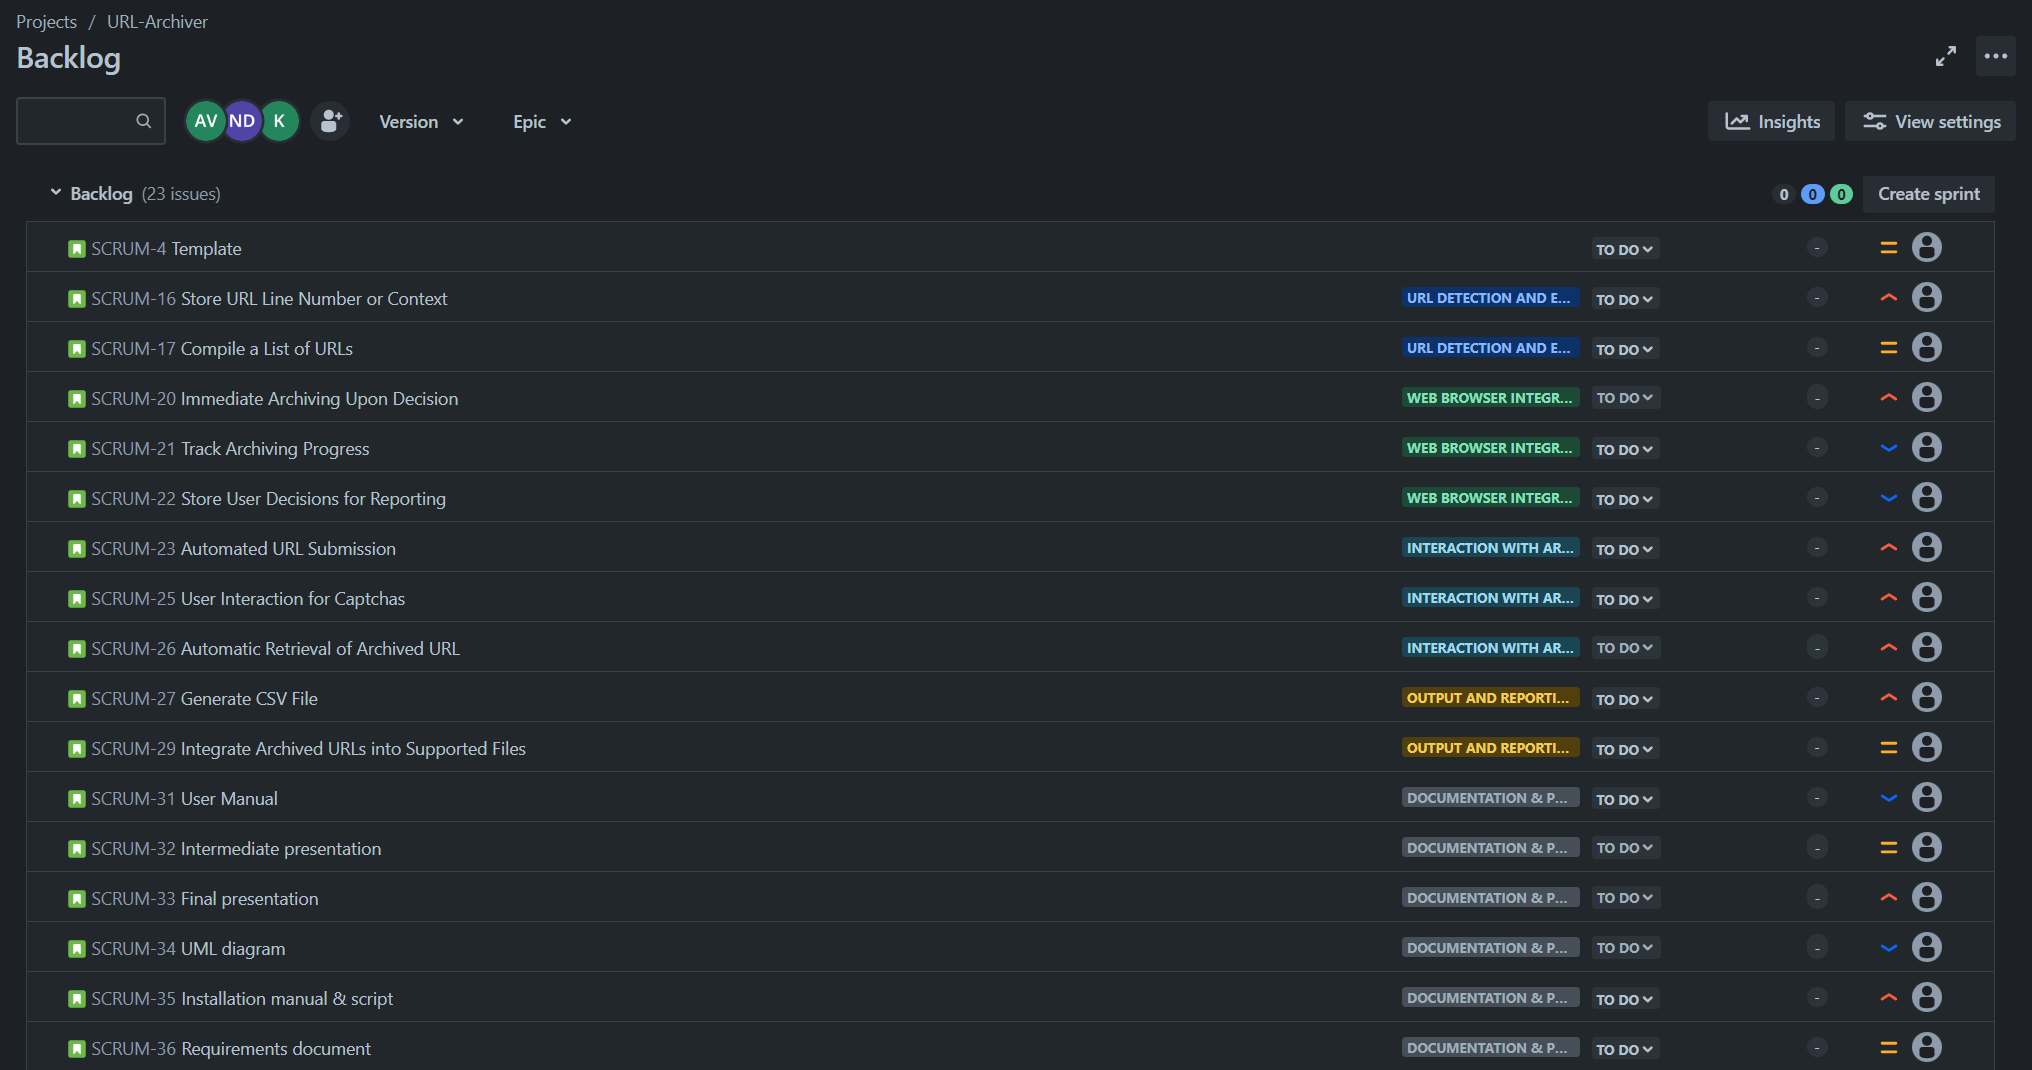
\includegraphics[width=1\textwidth]{pictures/backlog}
    \caption{Product Backlog}
    \label{fig:backlog}
\end{figure}

The prioritisation of user stories in the backlog is based on the business value field, which has a value between one and ten.
The business value is a vague estimate of how much value the individual user story has to the business, or in our case, to our stakeholders.
We endeavour to estimate the business value based on the expected importance of the function to the stakeholder.
The following priorities are possible:
\begin{itemize}
    \item Highest
    \item High
    \item Medium
    \item Low
    \item Lowest
\end{itemize}

\subsection{Sprint Backlogs}
Below we describe our recent and current sprints.
During the sprint planning we fill the respective sprint backlog with user stories that serve the sprint goal.
A user story must satisfy our Definition of Ready before it can be included in the sprint.
In addition, the stories must be estimated and the total number of story points must not exceed our defined velocity.

\subsubsection{Sprint 1}
Below is a screenshot of our board from the first sprint with the corresponding sprint goal.
\begin{figure}[h!]
    \centering
    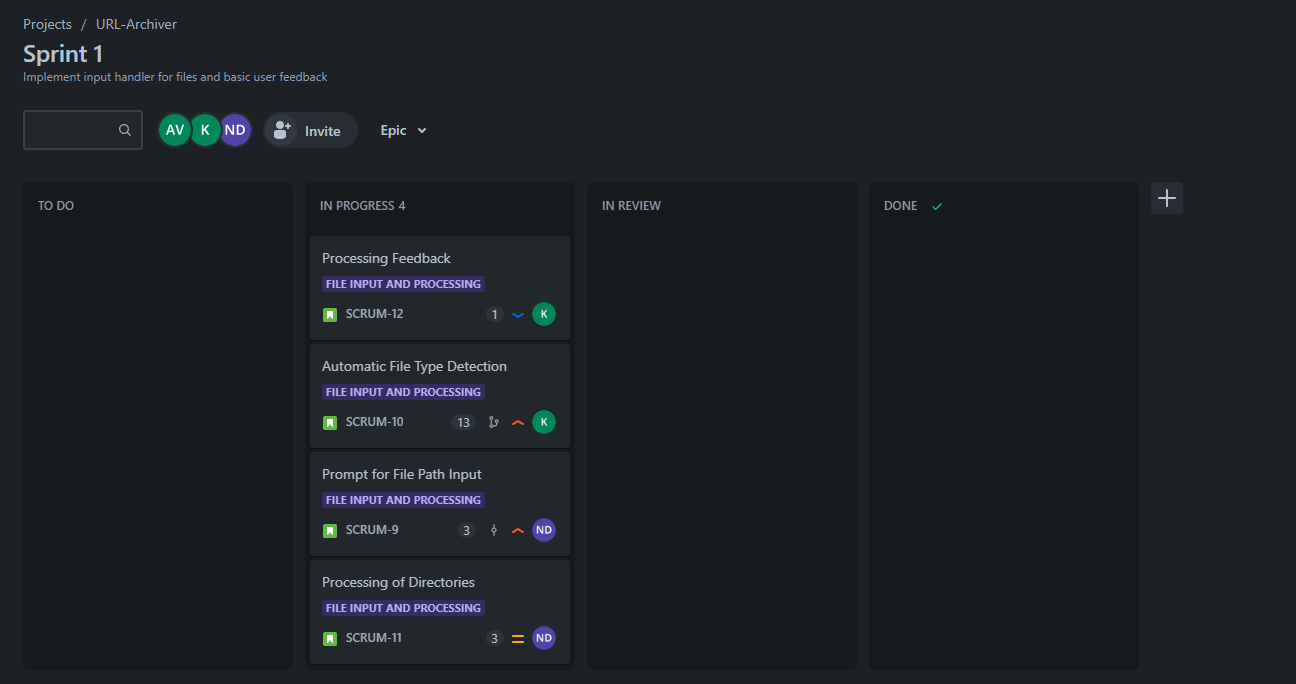
\includegraphics[width=1\textwidth]{pictures/backlog_sprint_1}
    \caption{Sprint 1 Backlog}
    \label{fig:backlog_sprint_1}
\end{figure}

The user stories from the first sprint are shown below. The stories have been estimated and prioritised.

\begin{figure}[h!]
    \centering
    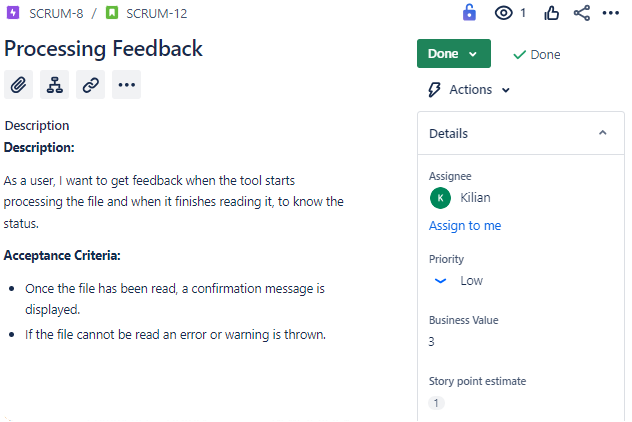
\includegraphics[width=1\textwidth]{pictures/Scrum/Sprint 1/UserStory_4}
    \caption{User Story Detail for "Processing Feedback"}
    \label{fig:sprint_1_userstory_1}
\end{figure}
\begin{figure}[h!]
    \centering
    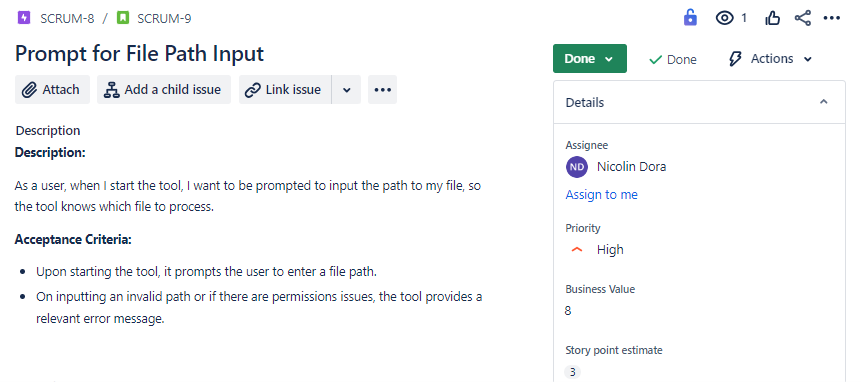
\includegraphics[width=1\textwidth]{pictures/Scrum/Sprint 1/UserStory_1}
    \caption{User Story Detail for "Prompt for file path input"}
    \label{fig:sprint_1_userstory_2}
\end{figure}
\begin{figure}[h!]
    \centering
    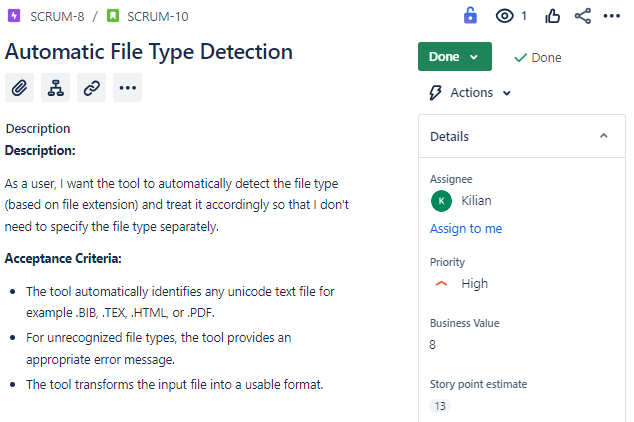
\includegraphics[width=1\textwidth]{pictures/Scrum/Sprint 1/UserStory_2}
    \caption{User Story Detail for "Automatic File Type Detection"}
    \label{fig:sprint_1_userstory_3}
\end{figure}
\begin{figure}[h!]
    \centering
    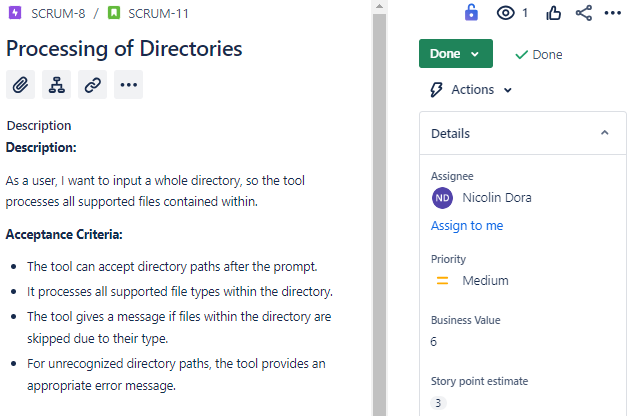
\includegraphics[width=1\textwidth]{pictures/Scrum/Sprint 1/UserStory_3}
    \caption{User Story Detail for "Processing of Directories"}
    \label{fig:sprint_1_userstory_4}
\end{figure}
\clearpage

In the first sprint, the burn down chart looks like this:
\begin{figure}[h!]
    \centering
    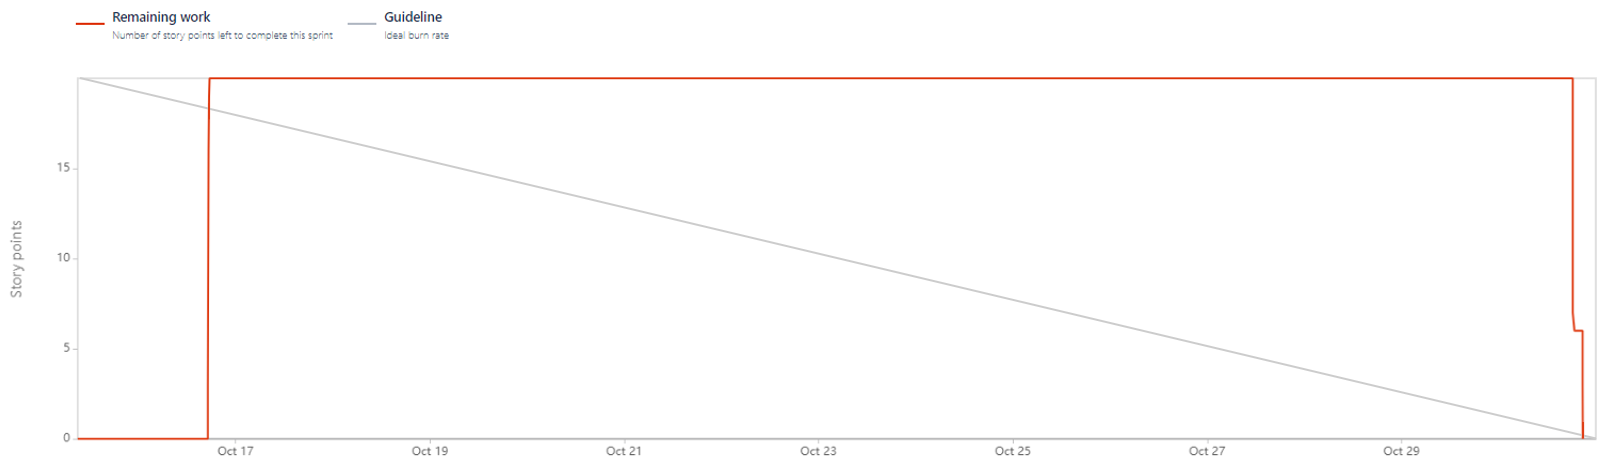
\includegraphics[width=1\textwidth]{pictures/Scrum/Sprint 1/sprint1_burndownchart}
    \caption{Sprint 1 Burn Up Chart}
    \label{fig:sprint_1_bunrdown_chart}
\end{figure}

The reason for this is that we did not create tasks for our user stories as they were small enough.
Furthermore, a code review for corresponding user stories could only be conducted towards the end of the sprint, resulting in the finalisation of user stories at that point.
\clearpage

\subsubsection{Sprint 2}
Below is a screenshot of our board from the second sprint with the corresponding sprint goal.
\begin{figure}[h!]
    \centering
    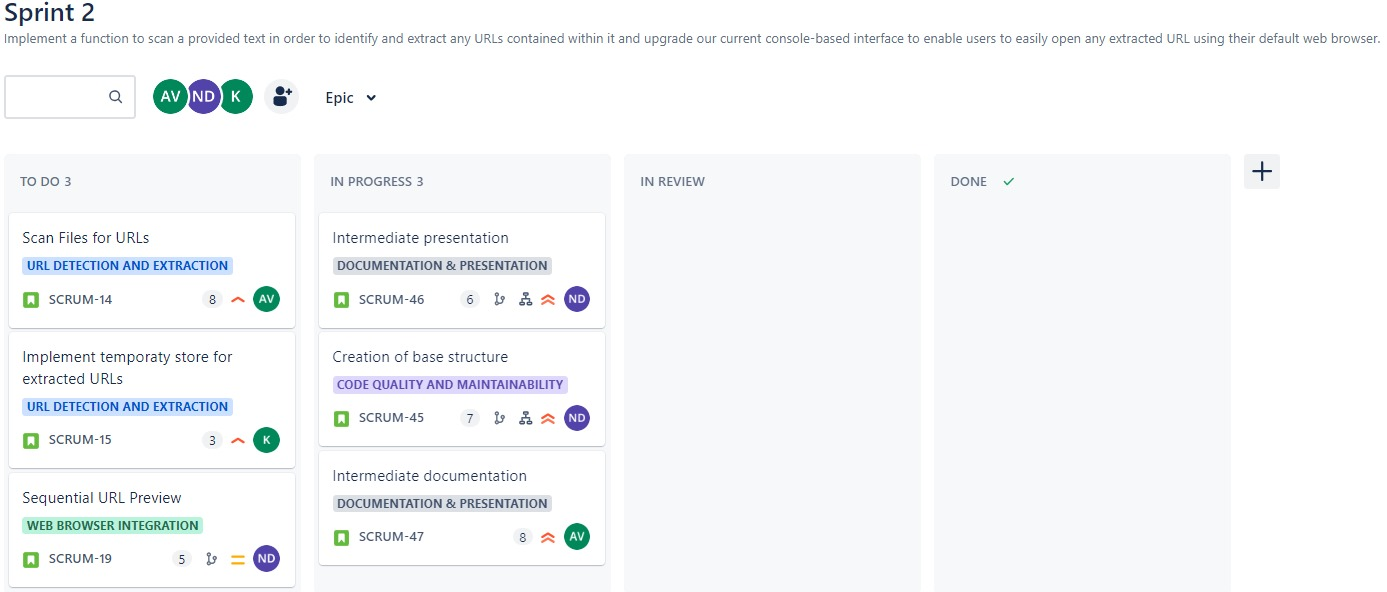
\includegraphics[width=1\textwidth]{pictures/Scrum/Sprint 2/Sprint2_Backlog}
    \caption{Sprint 2 Backlog}
    \label{fig:sprint_2_backlog}
\end{figure}

The user stories from the second sprint are shown below. The stories have been estimated and prioritised.
\begin{figure}[h!]
    \centering
    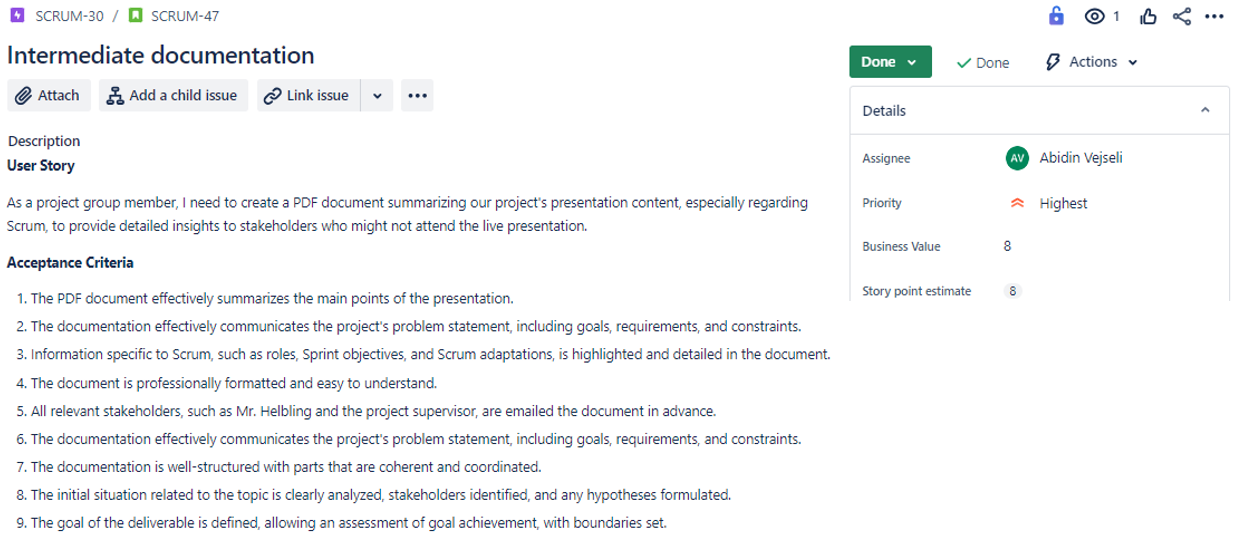
\includegraphics[width=1\textwidth]{pictures/Scrum/Sprint 2/UserStory_13}
    \caption{User Story Detail for "Intermediate Documentation"}
    \label{fig:sprint_2_userstory_1}
\end{figure}
\begin{figure}[h!]
    \centering
    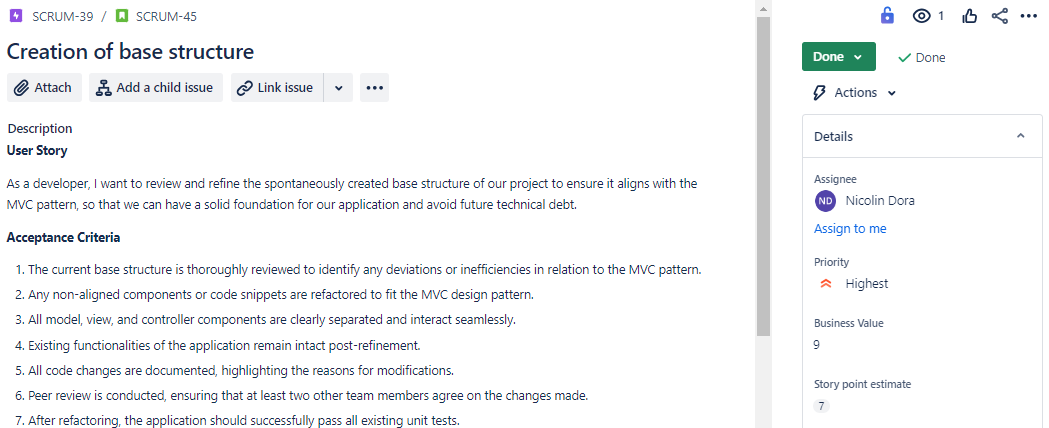
\includegraphics[width=1\textwidth]{pictures/Scrum/Sprint 2/UserStory_11}
    \caption{User Story Detail for "Creation of Base Structure"}
    \label{fig:sprint_2_userstory_2}
\end{figure}
\begin{figure}[h!]
    \centering
    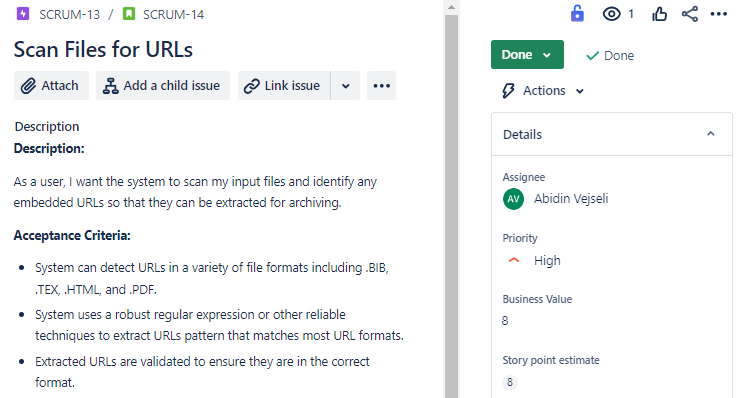
\includegraphics[width=1\textwidth]{pictures/Scrum/Sprint 2/UserStory_5}
    \caption{User Story Detail for "Scan Files for URLs"}
    \label{fig:sprint_2_userstory_3}
\end{figure}
\begin{figure}[h!]
    \centering
    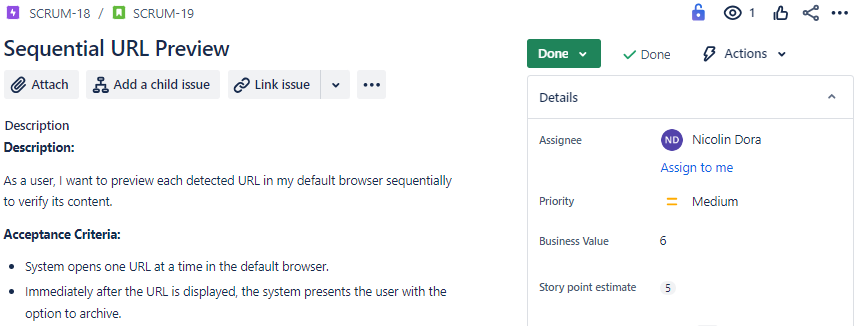
\includegraphics[width=1\textwidth]{pictures/Scrum/Sprint 2/UserStory_7}
    \caption{User Story Detail for "Sequential URL Preview"}
    \label{fig:sprint_2_userstory_4}
\end{figure}
\begin{figure}[h!]
    \centering
    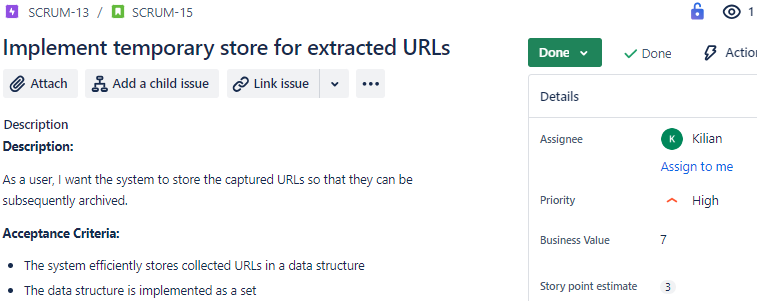
\includegraphics[width=1\textwidth]{pictures/Scrum/Sprint 2/UserStory_6}
    \caption{User Story Detail for "Implement temporary store for extracted URLs"}
    \label{fig:sprint_2_userstory_5}
\end{figure}
\begin{figure}[h!]
    \centering
    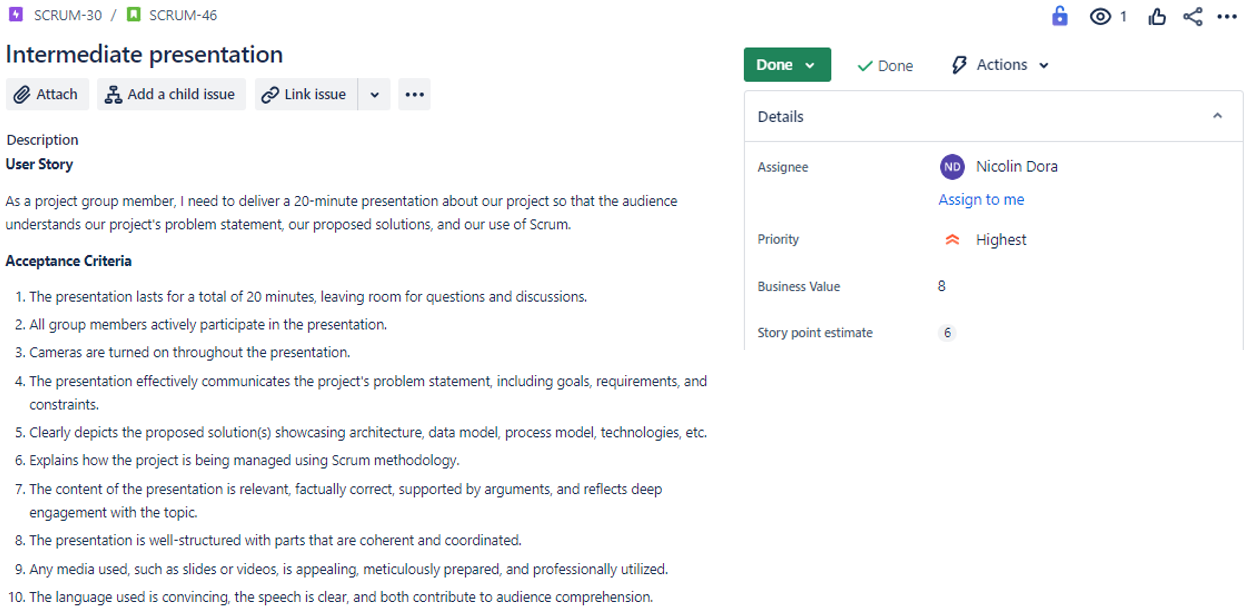
\includegraphics[width=1\textwidth]{pictures/Scrum/Sprint 2/UserStory_12}
    \caption{User Story Detail for "Intermediate presentation"}
    \label{fig:sprint_2_userstory_6}
\end{figure}
\clearpage

In the second sprint, the burn down chart looks like this:
\begin{figure}[h!]
    \centering
    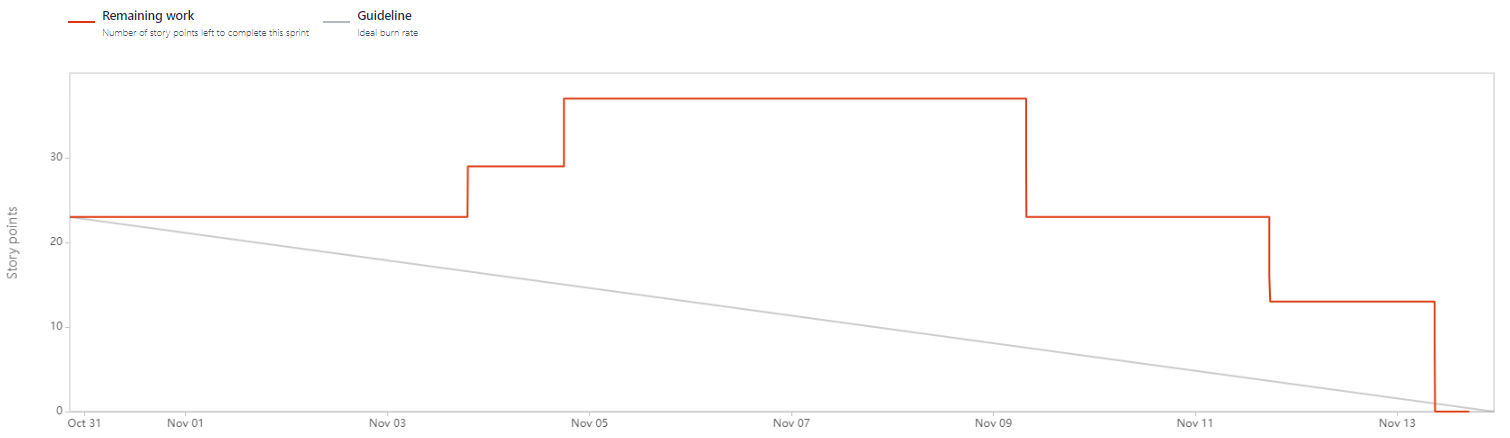
\includegraphics[width=1\textwidth]{pictures/Scrum/Sprint 2/Sprint2_burndownchart}
    \caption{Sprint 2 Burn Down Chart}
    \label{fig:sprint_2_bunrdown_chart}
\end{figure}

Compared to the initial sprint, our workload significantly increased, and we introduced new user stories after the sprint began.
Despite these additions, we maintained a strong pace and seamlessly managed the extra tasks that arose from the intermediate presentation and documentation requirements.
\clearpage


\subsubsection{Sprint 3}
Below is a screenshot of our board from the third sprint with the corresponding sprint goal.
\begin{figure}[h!]
    \centering
    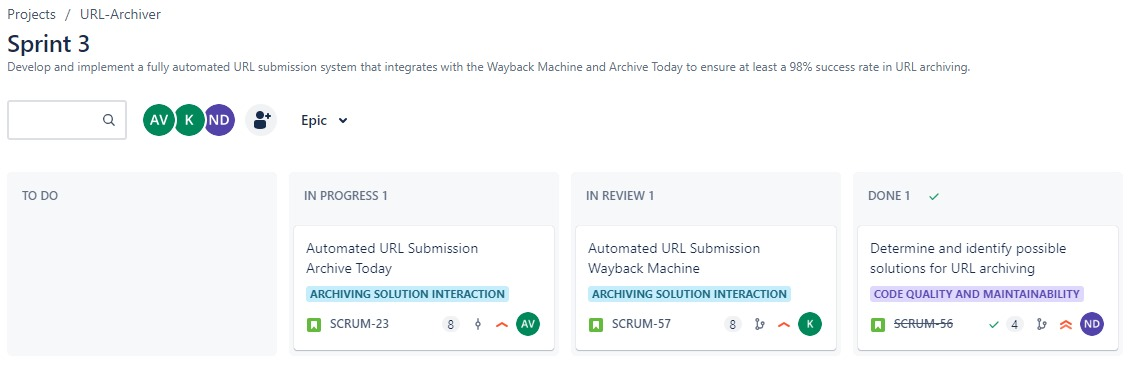
\includegraphics[width=1\textwidth]{pictures/Scrum/Sprint 3/Sprint3_Backlog}
    \caption{Sprint 3 Backlog}
    \label{fig:sprint_3_backlog}
\end{figure}

The user stories from the third sprint are shown below. The stories have been estimated and prioritised.
\begin{figure}[h!]
    \centering
    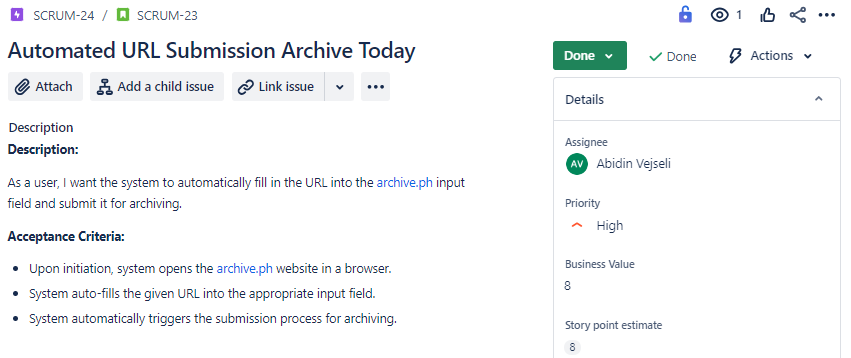
\includegraphics[width=1\textwidth]{pictures/Scrum/Sprint 3/UserStory_8}
    \caption{User Story Detail for "Intermediate Documentation"}
    \label{fig:sprint_3_userstory_1}
\end{figure}
\begin{figure}[h!]
    \centering
    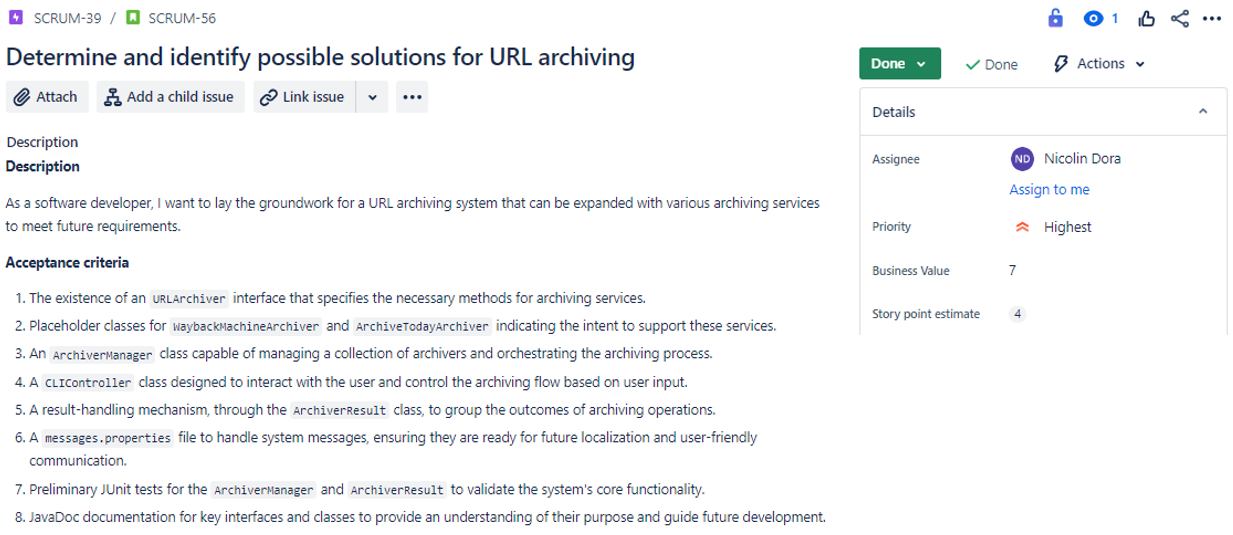
\includegraphics[width=1\textwidth]{pictures/Scrum/Sprint 3/UserStory_14}
    \caption{User Story Detail for "Creation of Base Structure"}
    \label{fig:sprint_3_userstory_2}
\end{figure}
\begin{figure}[h!]
    \centering
    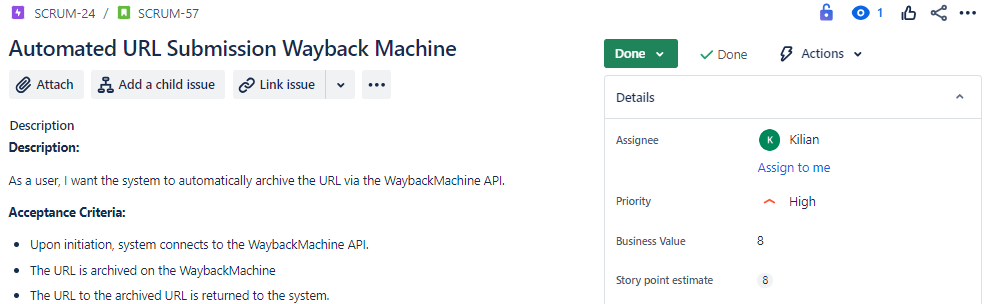
\includegraphics[width=1\textwidth]{pictures/Scrum/Sprint 3/UserStory_15}
    \caption{User Story Detail for "Scan Files for URLs"}
    \label{fig:sprint_3_userstory_3}
\end{figure}

In the third sprint, the burn down chart looks like this:
\begin{figure}[h!]
    \centering
    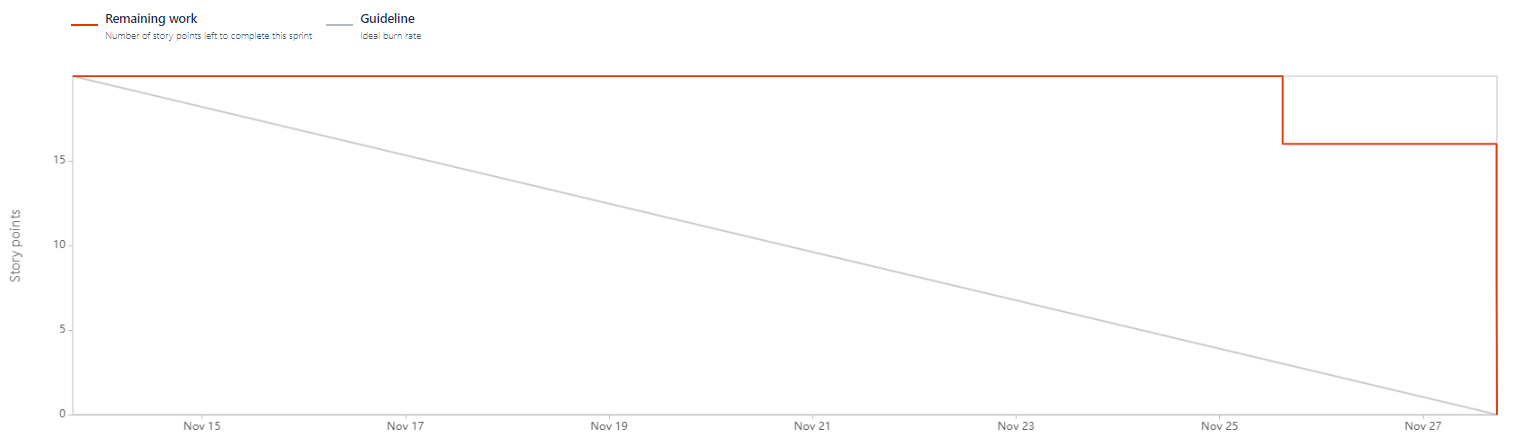
\includegraphics[width=1\textwidth]{pictures/Scrum/Sprint 3/Sprint3_burndownchart}
    \caption{Sprint 3 Burn Down Chart}
    \label{fig:sprint_3_bunrdown_chart}
\end{figure}

During the third sprint, our progress on user stories was limited to the completion of only three due to the 'special week 3'.
This meant that these stories had to be completed in the second half of the sprint due to the heavy workload of this special week.
The impact of this adaptation to our sprint schedule due to 'special week 3' is reflected in the trends seen in our burndown chart.
\clearpage

\subsubsection{Sprint 4}
Below is a screenshot of our board from the forth sprint.
\begin{figure}[h!]
    \centering
    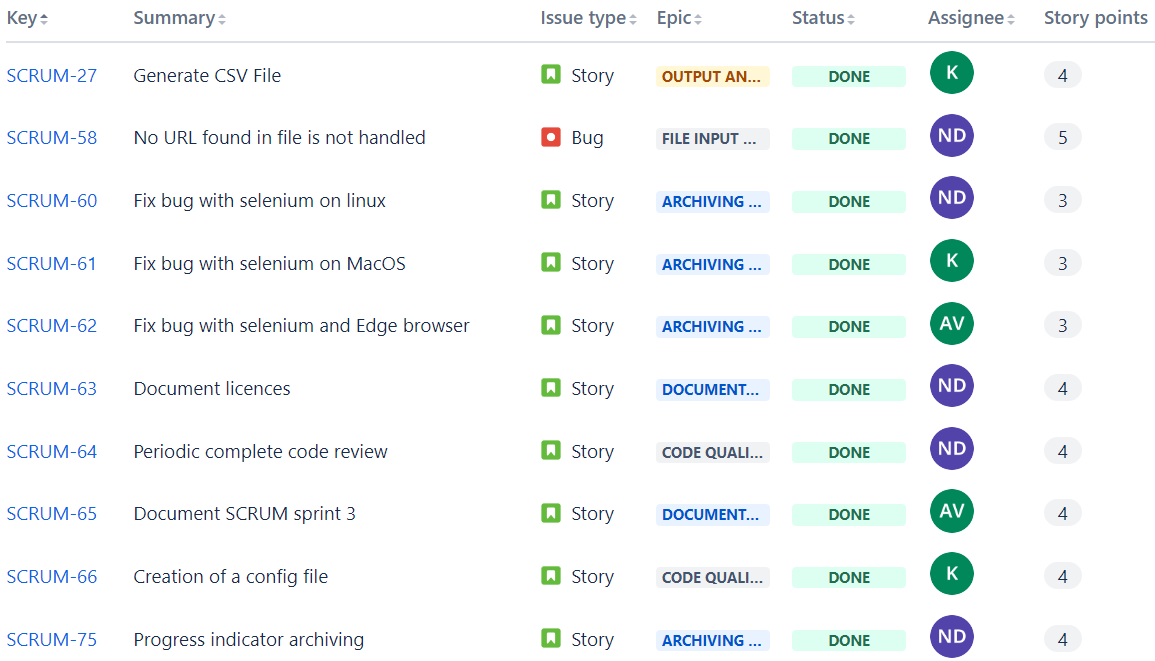
\includegraphics[width=1\textwidth]{pictures/Scrum/Sprint 4/Sprint4_Backlog}
    \caption{Sprint 4 Backlog}
    \label{fig:sprint_4_backlog}
\end{figure}

The user stories from the forth sprint are shown below. The stories have been estimated and prioritised.
\begin{figure}[h!]
    \centering
    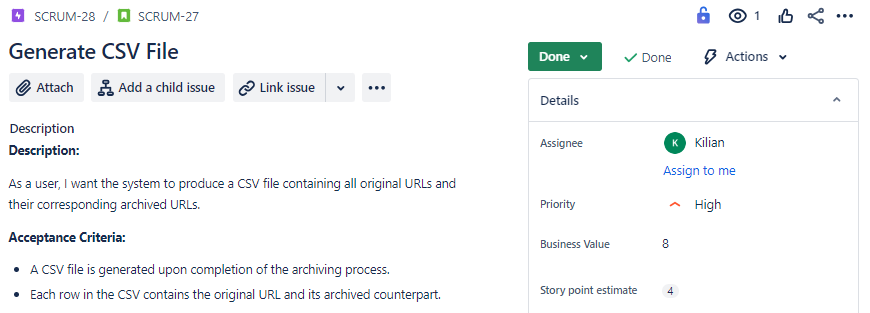
\includegraphics[width=1\textwidth]{pictures/Scrum/Sprint 4/UserStory_9}
    \caption{User Story Detail for "Generate CSV File"}
    \label{fig:sprint_4_userstory_1}
\end{figure}
\begin{figure}[h!]
    \centering
    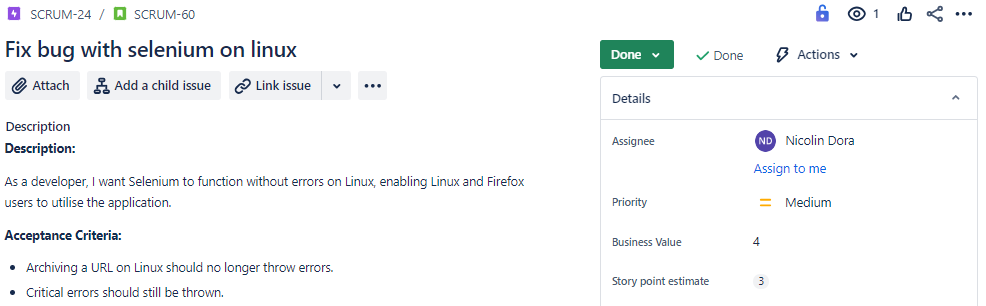
\includegraphics[width=1\textwidth]{pictures/Scrum/Sprint 4/UserStory_16}
    \caption{User Story Detail for "Fix bug with selenium on linux"}
    \label{fig:sprint_4_userstory_2}
\end{figure}
\begin{figure}[h!]
    \centering
    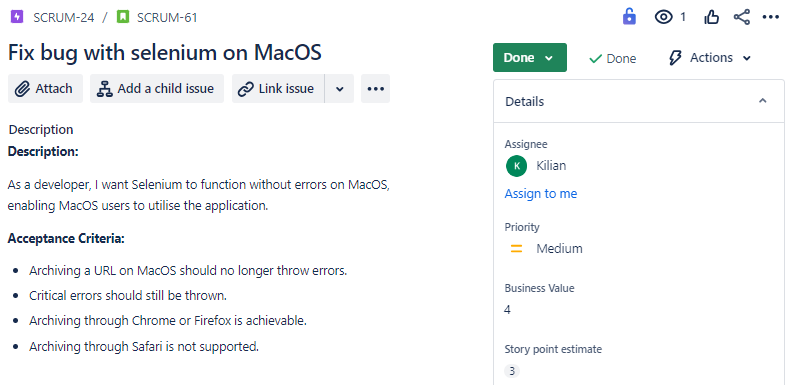
\includegraphics[width=1\textwidth]{pictures/Scrum/Sprint 4/UserStory_17}
    \caption{User Story Detail for "Fix bug with selenium on MacOS"}
    \label{fig:sprint_4_userstory_3}
\end{figure}
\begin{figure}[h!]
    \centering
    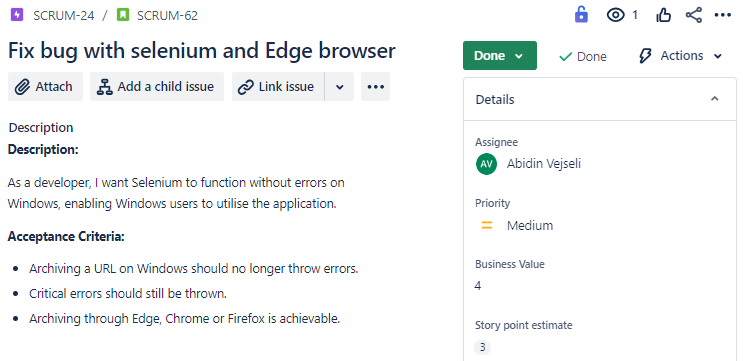
\includegraphics[width=1\textwidth]{pictures/Scrum/Sprint 4/UserStory_18}
    \caption{User Story Detail for "Fix bug With selenium and Edge browser"}
    \label{fig:sprint_4_userstory_4}
\end{figure}
\begin{figure}[h!]
    \centering
    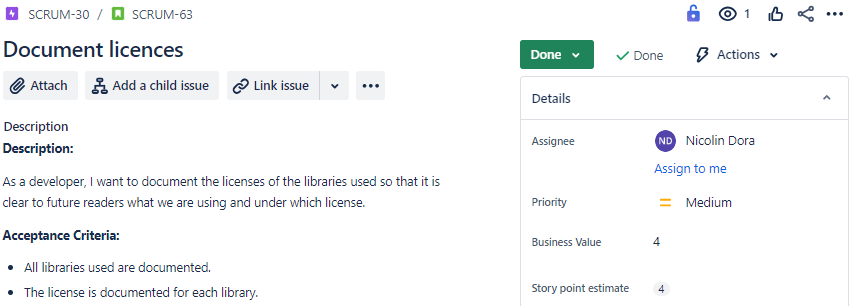
\includegraphics[width=1\textwidth]{pictures/Scrum/Sprint 4/UserStory_19}
    \caption{User Story Detail for "Document licences"}
    \label{fig:sprint_4_userstory_5}
\end{figure}
\begin{figure}[h!]
    \centering
    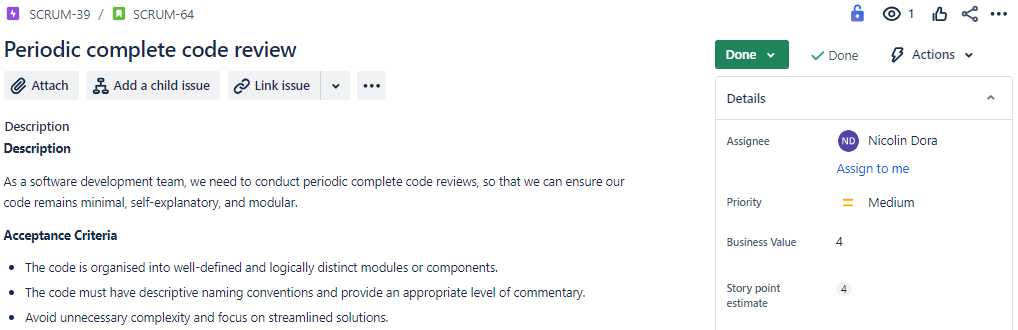
\includegraphics[width=1\textwidth]{pictures/Scrum/Sprint 4/UserStory_20}
    \caption{User Story Detail for "Periodic complete code review"}
    \label{fig:sprint_4_userstory_6}
\end{figure}
\begin{figure}[h!]
    \centering
    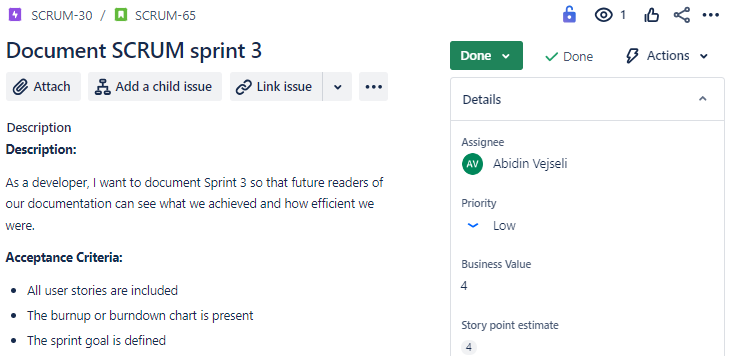
\includegraphics[width=1\textwidth]{pictures/Scrum/Sprint 4/UserStory_21}
    \caption{User Story Detail for "Document SCRUM sprint 3"}
    \label{fig:sprint_4_userstory_7}
\end{figure}
\begin{figure}[h!]
    \centering
    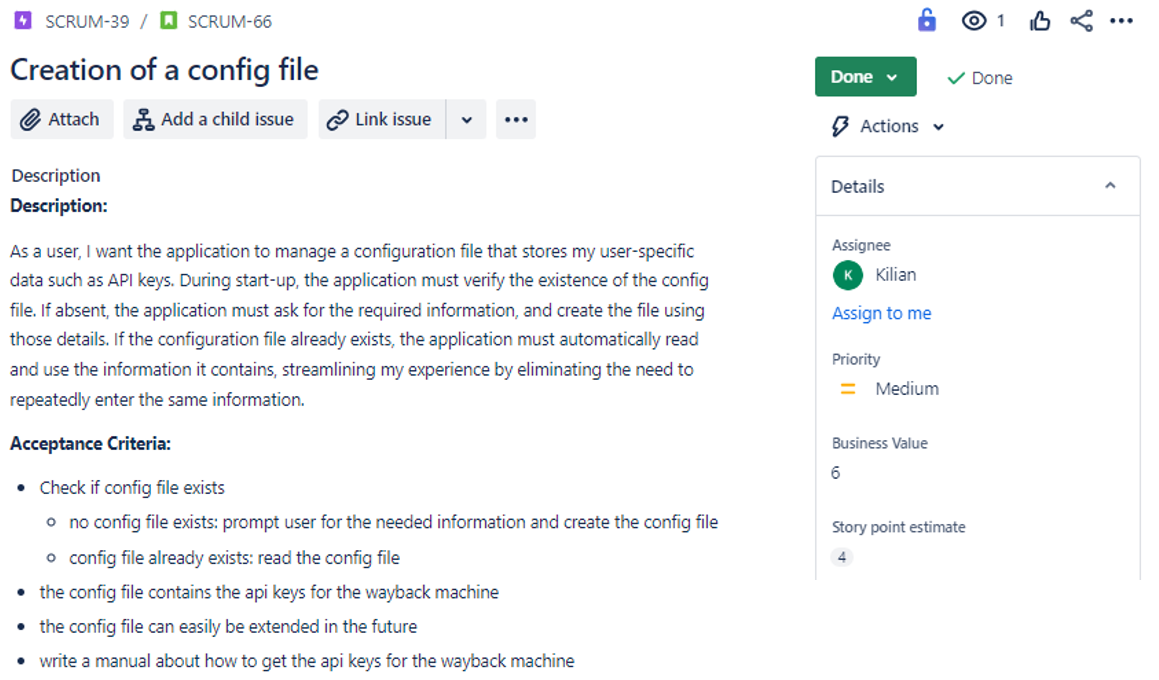
\includegraphics[width=1\textwidth]{pictures/Scrum/Sprint 4/UserStory_22}
    \caption{User Story Detail for "Creation of a config file"}
    \label{fig:sprint_4_userstory_8}
\end{figure}
\begin{figure}[h!]
    \centering
    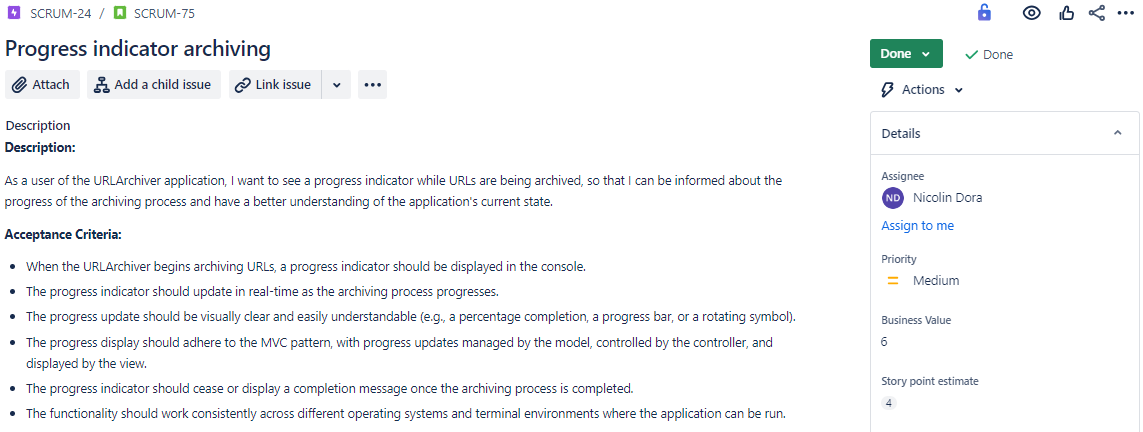
\includegraphics[width=1\textwidth]{pictures/Scrum/Sprint 4/UserStory_24}
    \caption{User Story Detail for "Progress indicator archiving"}
    \label{fig:sprint_4_userstory_9}
\end{figure}
\begin{figure}[h!]
    \centering
    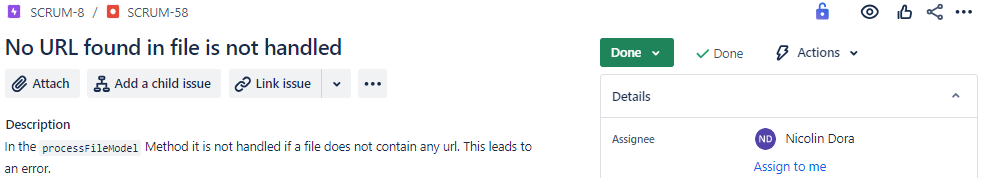
\includegraphics[width=1\textwidth]{pictures/Scrum/Sprint 4/Bug_1}
    \caption{Bug Detail for "No URL found in file is not handled"}
    \label{fig:sprint_4_bug_1}
\end{figure}


In the forth sprint, the burn down chart looks like this:
\begin{figure}[h!]
    \centering
    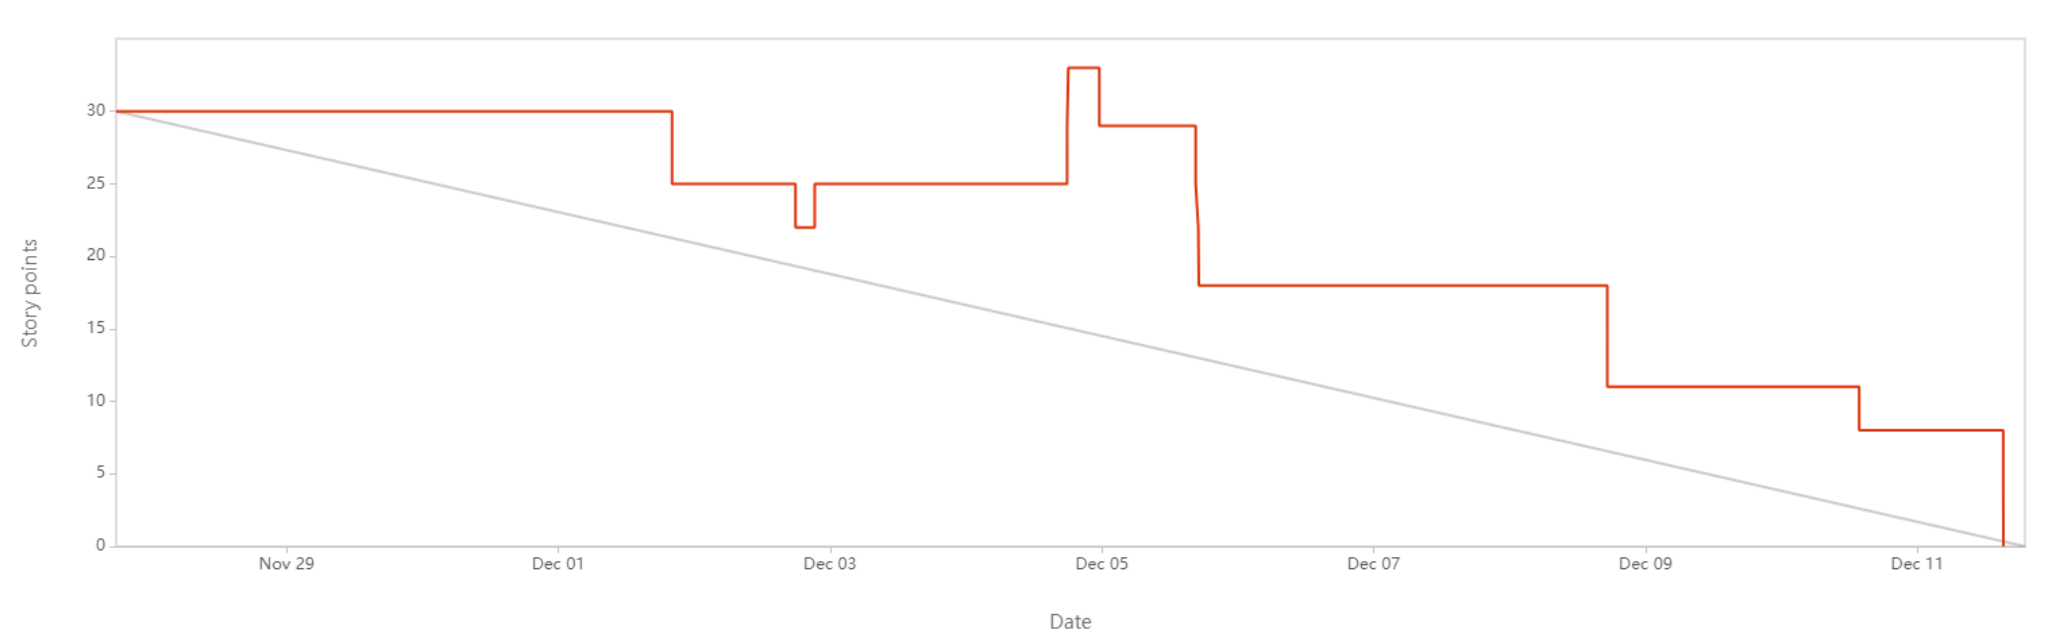
\includegraphics[width=1\textwidth]{pictures/Scrum/Sprint 4/Sprint4_Burndownchart}
    \caption{Sprint 4 Burn Down Chart}
    \label{fig:sprint_4_bunrdown_chart}
\end{figure}

Compared to the previous sprint, we were more efficient and successfully accommodated additional user stories that were initiated after the sprint began.
The completion of all allocated user stories within the sprint timeframe demonstrates our solid teamwork and sprint management capabilities.
\clearpage


\subsubsection{Sprint 5}
Below is a screenshot of our board from the fifth sprint.
\begin{figure}[h!]
    \centering
    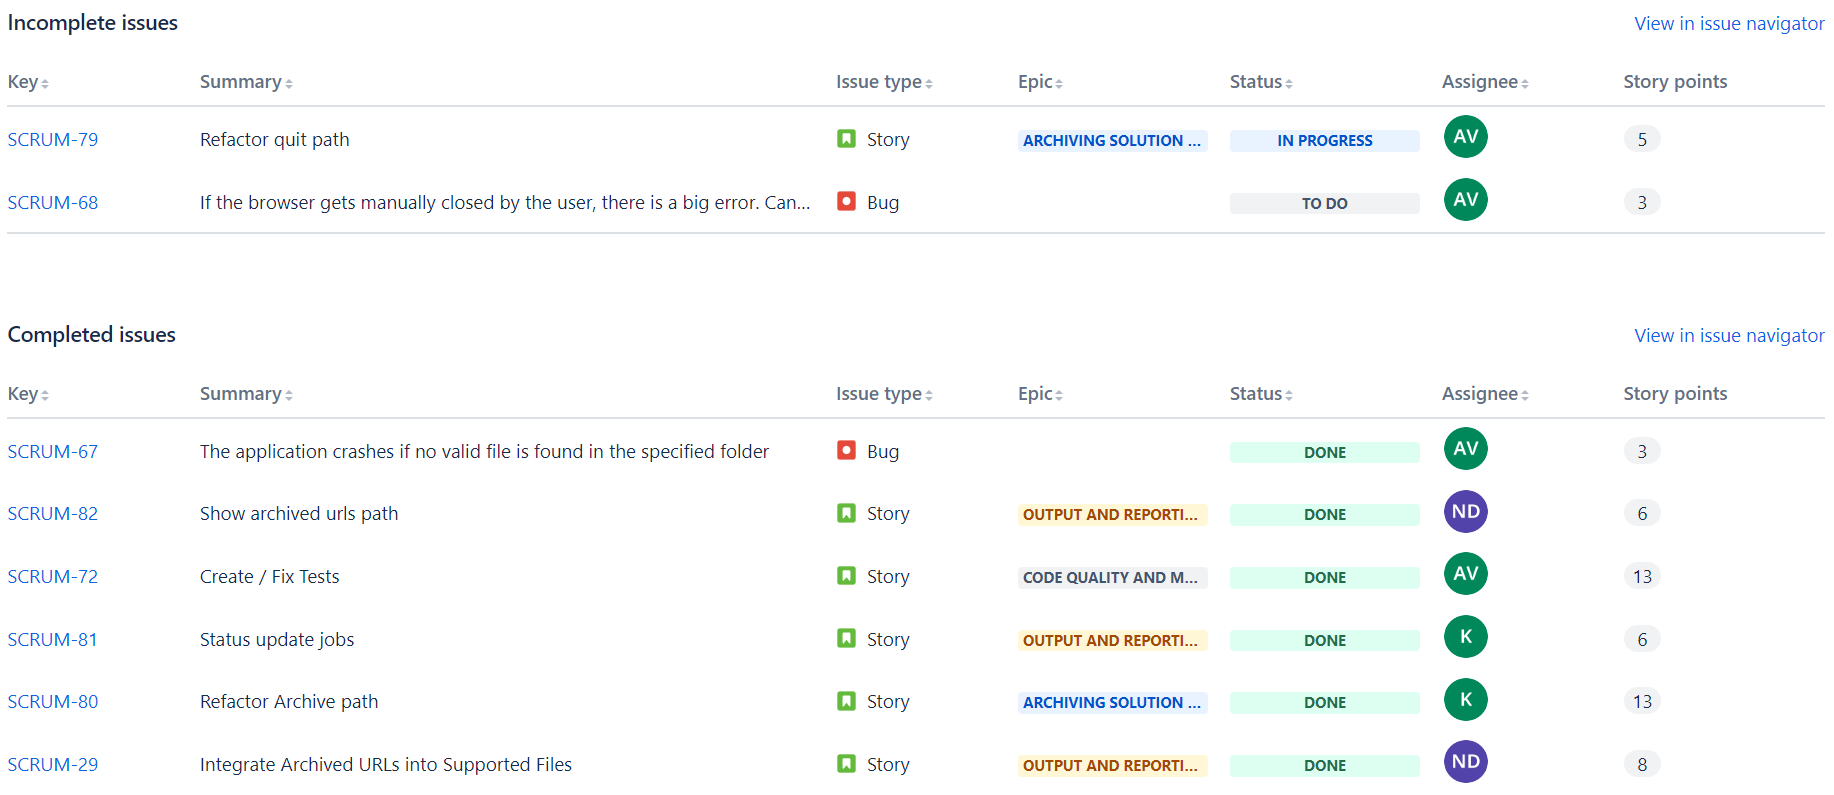
\includegraphics[width=1\textwidth]{pictures/Scrum/Sprint 5/Sprint5_Backlog}
    \caption{Sprint 5 Backlog}
    \label{fig:sprint_5_backlog}
\end{figure}

The user stories from the fifth sprint are shown below. The stories have been estimated and prioritised.
\begin{figure}[h!]
    \centering
    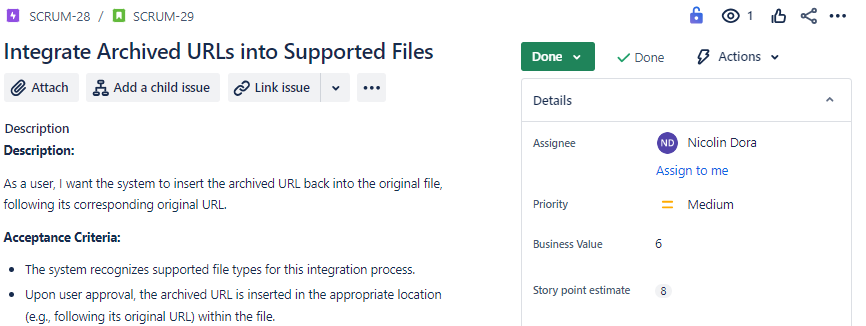
\includegraphics[width=1\textwidth]{pictures/Scrum/Sprint 5/UserStory_10}
    \caption{User Story Detail for "Integrate Archived URLs into Supported Files"}
    \label{fig:sprint_5_userstory_1}
\end{figure}
\begin{figure}[h!]
    \centering
    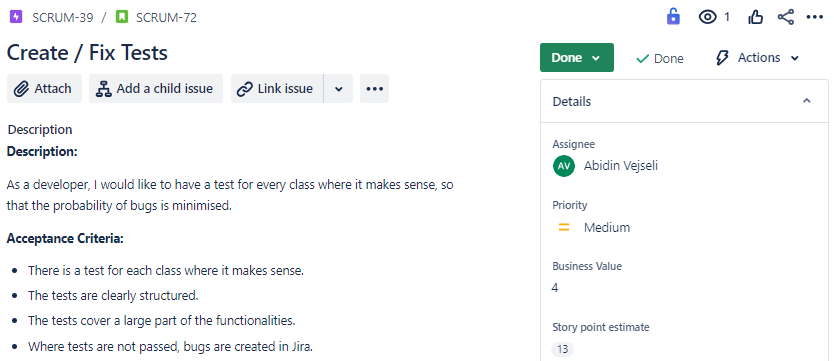
\includegraphics[width=1\textwidth]{pictures/Scrum/Sprint 5/UserStory_23}
    \caption{User Story Detail for "Create / Fix Tests"}
    \label{fig:sprint_5_userstory_2}
\end{figure}
\begin{figure}[h!]
    \centering
    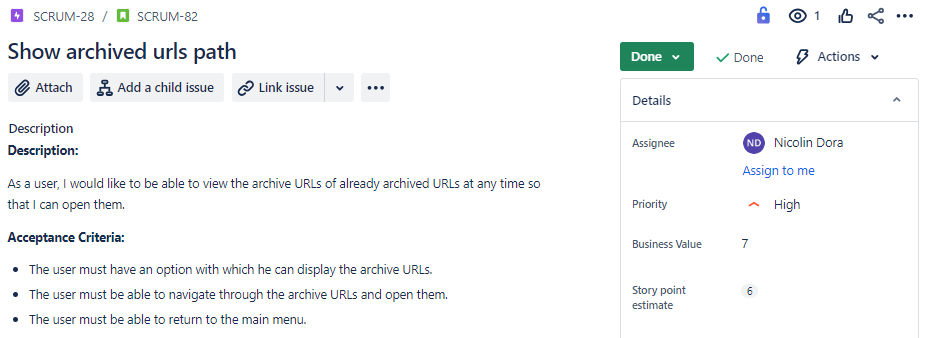
\includegraphics[width=1\textwidth]{pictures/Scrum/Sprint 5/UserStory_25}
    \caption{User Story Detail for "Show archived urls path"}
    \label{fig:sprint_5_userstory_3}
\end{figure}

In the fifth sprint, the burn down chart looks like this:
\begin{figure}[h!]
    \centering
    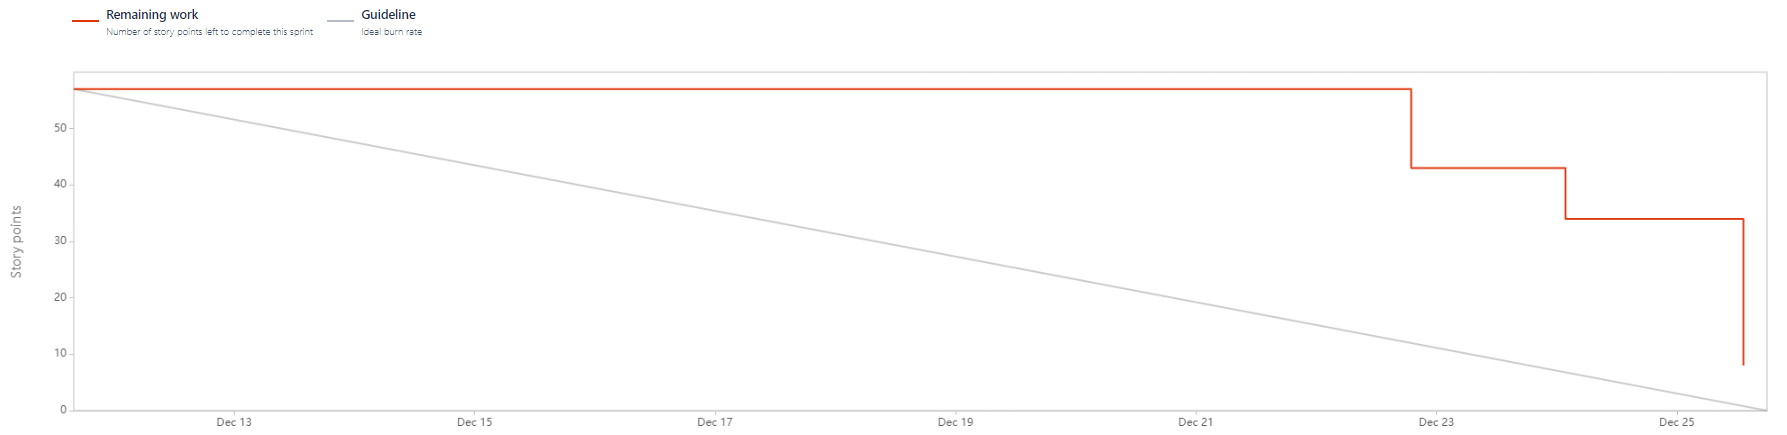
\includegraphics[width=1\textwidth]{pictures/Scrum/Sprint 5/Sprint5_Burndownchart}
    \caption{Sprint 5 Burn Down Chart}
    \label{fig:sprint_5_bunrdown_chart}
\end{figure}

In sprint 5, our time was limited due to commitments in other modules and the upcoming Christmas period, which resulted in team member absences.
We encountered an unexpected challenge with the extensive time required for test refactoring, as we prioritise quality, which often demands more time.
As a result, we were unable to complete all planned user stories and had to carry them over to the next sprint.
These challenges are reflected in the burn down chart.
\clearpage


\section{Scrum Adaptionen}
As part of Project 1, we have adjusted Scrum in order to use it in the best possible way. The adjustments are explained in this chapter.

\subsection{Definition of Ready (DOR)}
Our DOR includes conditions that ensure that all team members understand the user stories and know when a user story can be included in a sprint. The DOR was set in line with the INVEST\footnote{\href{https://xp123.com/articles/invest-in-good-stories-and-smart-tasks/}{XP123 article: Invest in good stories and smart tasks}} criteria. A user story in the product backlog must meet the DOR before it can be included in a sprint.

\textbf{Definition of Ready}
\begin{itemize}
    \item Ensure a clear definition
    \item Define the functionality or requirement to be implemented
    \item Clearly defined and testable acceptance criteria
    \item Ensure there are no or minimal dependencies
    \item Understood by the whole team
    \item The user story has been estimated
    \item The scope of the user story is small enough that it can be implemented in a single sprint.
\end{itemize}

\subsection{Definition of Done (DOD)}
Our DOD contains all the characteristics and standards that a user story must meet to be considered complete.
Once it satisfies the necessary quality requirements (acceptance criteria), the story can be considered complete and can be closed.
The goal of our DOD is to create transparency so that everyone has a common understanding of when a story can be closed.
A story that does not comply with the DOD may not be finalised.

\textbf{Definition of Done}
\begin{itemize}
    \item Coding standards and best practices are implemented
    \item Unit tests for the feature are written and passe
    \item Any changes to the code or functionality are documented
    \item The code and functionality are reviewed by peers
    \item The feature works across multiple platforms
    \item Code is integrated with master branch
    \item Documentation has been updated
    \item Acceptance criteria are met
\end{itemize}
\clearpage

\subsection{User Story Template}
For the creation of a user story, we have defined a template so that the user stories contain all the necessary information. Below is a screenshot of our template. It includes all the relevant fields for us: Assignee, Priority, Business Value, Story Points estimate and assigned Sprint. Furthermore, we describe the user story in the "Description" field in the format "AS A <user role> I WANT TO <the goal> [SO THAT <reason>]" as well as the Acceptance Criteria.
To ensure that we always have the DOR and DOD to hand, we also work with the Jira On-the-Fly add-on, which enables us to record both for each user story and tick off the individual points accordingly when they have been completed. This allows us to immediately recognise whether a user story can be included in a sprint and whether a story has been fully completed.
\begin{figure}[h!]
    \centering
    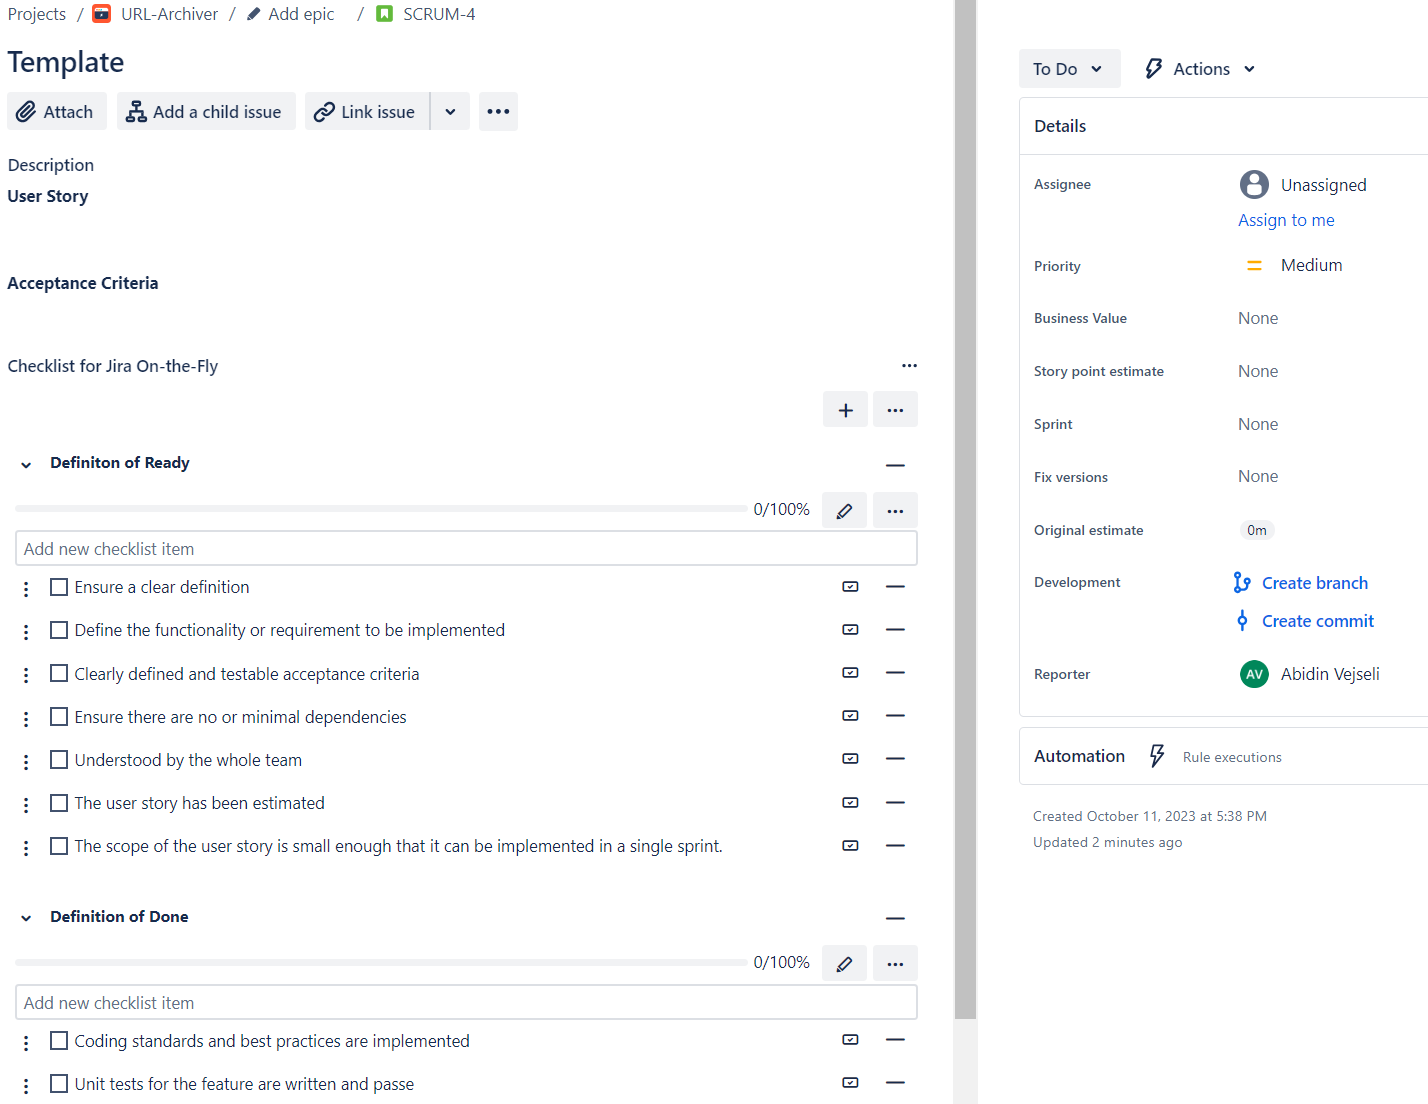
\includegraphics[width=1\textwidth]{pictures/Scrum/userstory_template}
    \caption{Screenshot from the user story template.}
    \label{fig:user_story_template}
\end{figure}
\clearpage

\subsection{Estimation method}
We have chosen the "T-shirt sizes" method because it is a simple way to estimate effort (story points). This method is based on the fact that everyone knows T-shirt sizes and that large sizes mean more work than small sizes. As a result, this method enables us to make efficient estimations, despite the lack of shared experience in the team.

Below is the scale we use:
\begin{figure}[h!]
    \centering
    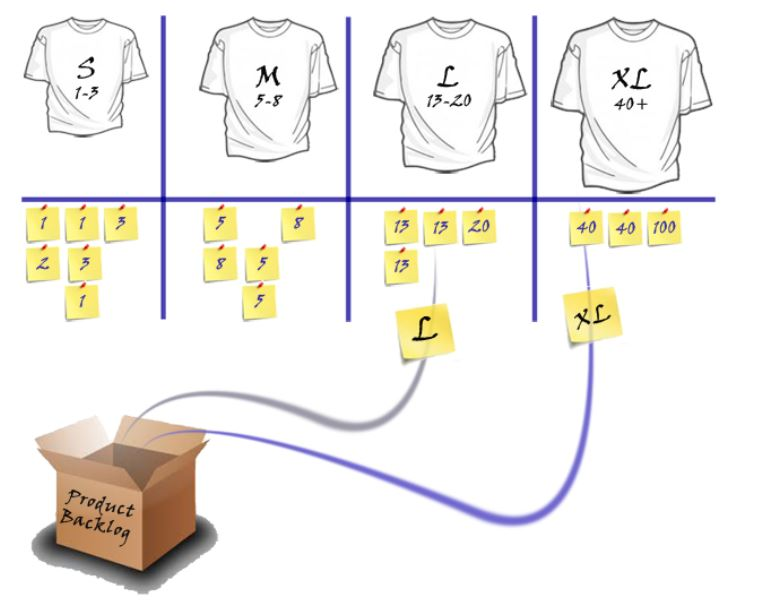
\includegraphics[width=1\textwidth]{pictures/tshirt_sizes}
    \caption{Ilustration of T-Shirt Sizes}
    \label{fig:tshirt_sizes}
\end{figure}
\clearpage

\subsection{Velocity}
To select the user stories and tasks to be worked on, a suitable criterion, velocity, is applied to estimate what can be completed in the upcoming sprint.

We have decided that we have a velocity of 30 story points per sprint.
Therefore, our workload per sprint should not exceed this threshold. We consciously take this into account during sprint planning.

\subsection{Sprint}
As a team, we have decided that our sprints will take place at two-week intervals. For each sprint we define a SMART sprint goal, which specifies the relevant user stories.

We decided in favour of the two-week rhythm because regular feedback is important to us and thus creates a greater learning effect. Additionally, we ascertained that one-week sprints would result in excessive overheads due to the administrative work involved in Scrum. Likewise, we consider sprints longer than two weeks to be impractical, as the interaction would suffer.

\subsubsection{Sprint Planning}
As part of sprint planning, we make decisions about which user stories can be implemented based on the sprint goal, the story points and the velocity.
Before a user story can be included in the sprint, it must be estimated by the Scrum team. This task is always carried out at the start of our sprint planning.
A sprint goal is then defined based on the estimated and prioritised user stories.
The user stories we select for the sprint are based on the business value, priority, story points and velocity of the team.
The sprint planning takes place on the first Monday of each sprint.
We have decided not to have a second sprint planning as we have already defined in our DOR that the user stories should be as small as possible. In addition, each developer has the opportunity to divide their user stories into tasks within the sprint. This allows a better overview of the progress in the sprint.

\subsubsection{Daily Scrum}
As a team, we have decided not to have daily Scrum meetings, as this is not possible because all team members do work part times. Instead, we have two weekly meetings (weeklys), on Wednesday and Friday at 17:00, which last a maximum of 15 minutes.
In addition, we have chosen to hold the meetings through Microsoft Teams as it is easier to organise.
The goal of these meetings is to share the current progress, address issues, update the team and briefly discuss the next steps.

\subsubsection{Sprint Review}
In the sprint review, we check the intermediate result of the processed user stories. We check whether all the stories that should be completed meet the DOD. Furthermore, we discuss in the team what went well, what problems we encountered and how we solved them. Based on these results, the product increment is created.
In our case, the product owner, who represents the customer, tests the product increment against the requirements. The review is done from the customer's perspective by testing the product increment. The outcomes are utilized to update the product backlog.
The sprint review meeting takes place on the last day of the sprint.

\subsubsection{Sprint Retrospective}
In the sprint retrospective, we gather information as a team about what went well and what didn't go as planned in the previous sprint.
We then derive specific improvements and plan their implementation. Our goal is to improve the efficiency, quality, communication and speed within our team. To achieve this, we give ourselves constructive criticism and are open to feedback.
The sprint retrospective takes place on the last day of the sprint.